%%%%%%%%%%%%%%%%%%%%%%%%%%%%%%%%%%%%%%%%%%%%%%%%%%%
%
%  New template code for TAMU Theses and Dissertations starting Fall 2016.  
%
%
%  Author: Sean Zachary Roberson
%  Version 3.17.09
%  Last Updated: 9/21/2017
%
%%%%%%%%%%%%%%%%%%%%%%%%%%%%%%%%%%%%%%%%%%%%%%%%%%%
%%%%%%%%%%%%%%%%%%%%%%%%%%%%%%%%%%%%%%%%%%%%%%%%%%%%%%%%%%%%%%%%%%%%%%
%%                           TIME TO SOLUTION ESTIMATOR CHAPTER
%%%%%%%%%%%%%%%%%%%%%%%%%%%%%%%%%%%%%%%%%%%%%%%%%%%%%%%%%%%%%%%%%%%%%



\chapter{TIME-TO-SOLUTION ESTIMATOR \label{cha:tts}}

This chapter is for the time to solution estimator description.

\section{Method}
The detailed method description will go here.

\section{2D Verification}

A verification study in 2D was run to verify the time-to-solution estimator for 2D partitioning schemes with perfectly balanced partitions. The test problems were verified against a code written by Jean Ragusa that mimics PDT's scheduler in two dimensions. For consistency, the time-to-solution estimator utilized an unweighted depth-of-graph algorithm during the verification study to match PDT's scheduling. The verification study consisted of the following problems:
\begin{enumerate}
	\item 2x2 to 10x10 subsets in x and y with regular partitions and 1 to 6 angles per quadrant.
	\item 2x2 to 10x10 subsets in x and y with mildly random partitions and 1 to 6 angles per quadrant.
	\item  2x2 to 10x10 subsets in x and y with random partitions and 1 to 6 angles per quadrant.
	\item  2x2 to 10x10 subsets in x and y with probable worst-case partitions and 1 to 6 angles per quadrant.
\end{enumerate}

"Mildly random" partitions keep the cut lines uniformly distributed in x, while the y cut lines vary slightly around the uniformly distributed cut lines of the regular partitions. Figure \ref{mild_random_partitions} shows an example of this. "Random" partitions possesses no such limitations on either set of cut lines, as shown by Fig. \ref{random_partitions}.

\subsection{Regular Partitions}

%Regular partitions
\begin{figure}[H]
\centering
\begin{subfigure}[b]{0.45\textwidth}
  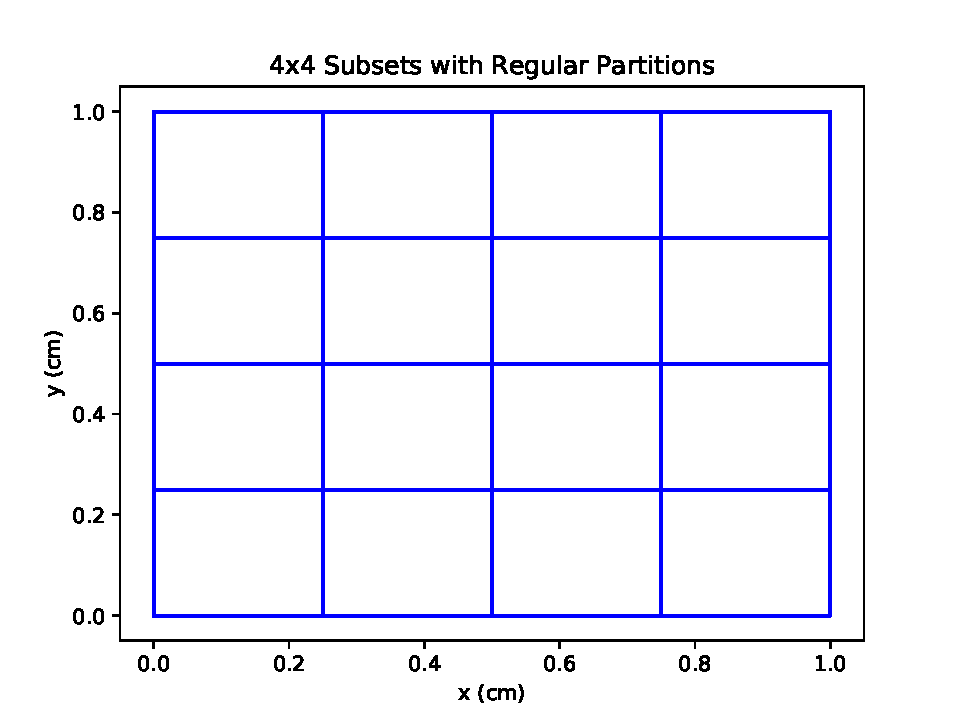
\includegraphics[width=\textwidth]{../cut_line_files/4_regular.pdf}
  \caption{4x4 subsets with regular partitions.}
  \label{4regular}
\end{subfigure}
\begin{subfigure}[b]{0.45\textwidth}
  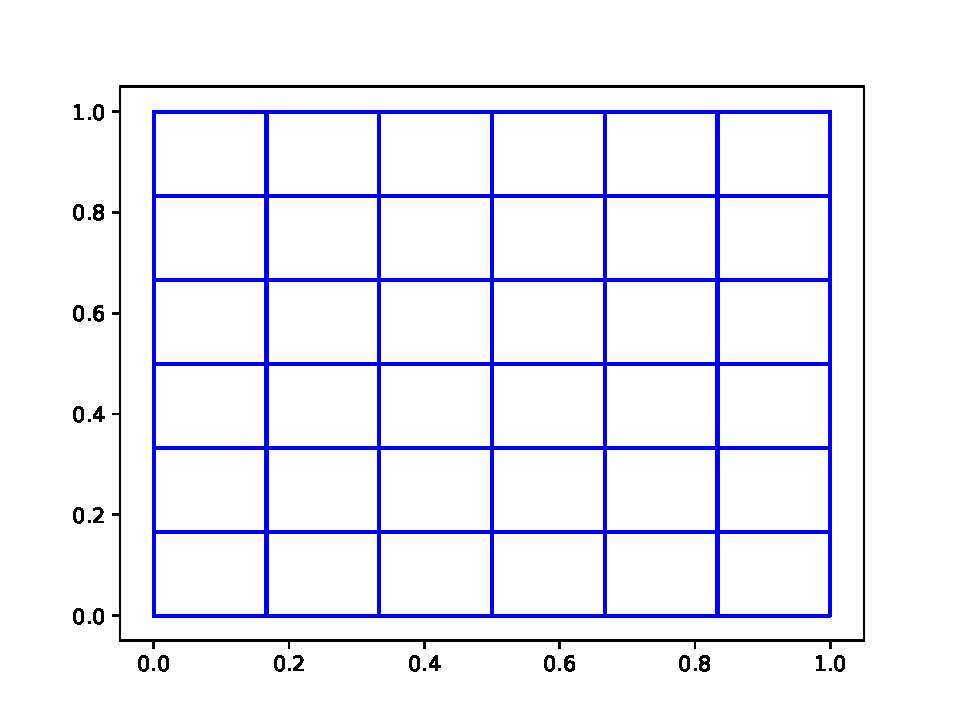
\includegraphics[width=\textwidth]{../cut_line_files/6_regular.pdf}
  \caption{6x6 subsets with regular partitions.}
  \label{6regular}
\end{subfigure}

\begin{subfigure}[b]{0.45\textwidth}
  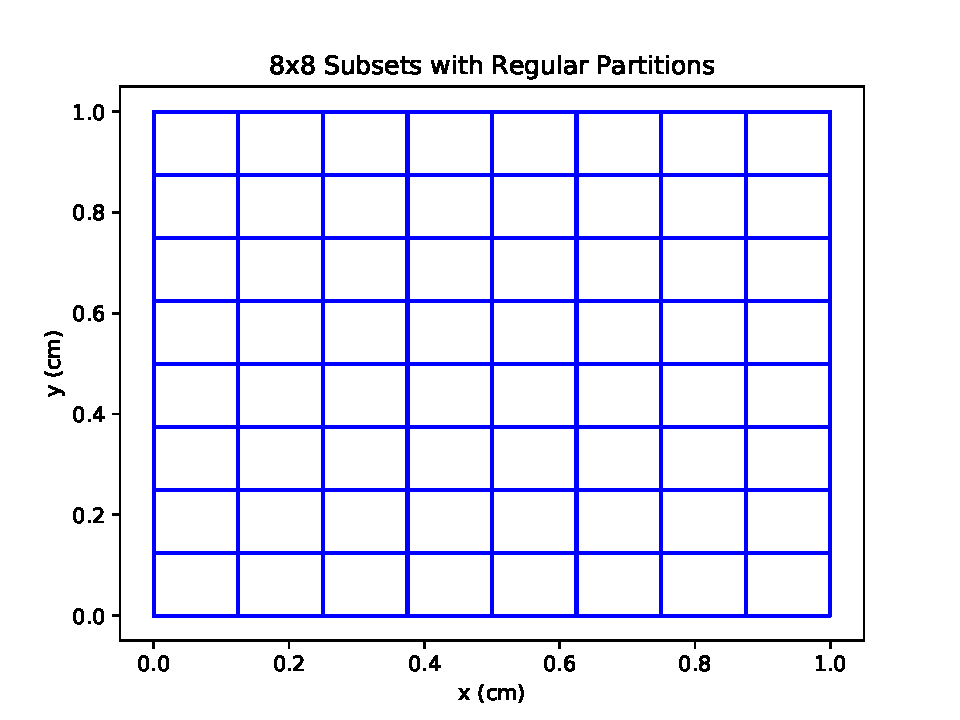
\includegraphics[width=\textwidth]{../cut_line_files/8_regular.pdf}
  \caption{8x8 subsets with regular partitions.}
  \label{8regular}
\end{subfigure}
\begin{subfigure}[b]{0.45\textwidth}
  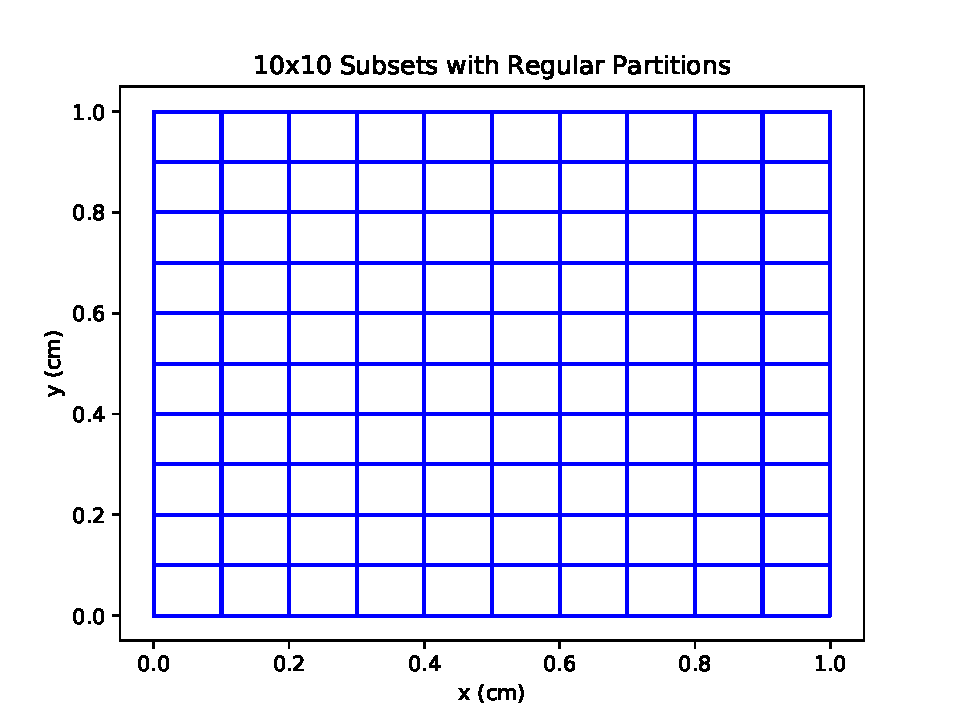
\includegraphics[width=\textwidth]{../cut_line_files/10_regular.pdf}
  \caption{10x10 subsets with regular partitions.}
  \label{10regular}
\end{subfigure}
\caption{Examples of regular partitioning.}
\label{regular_partitions}
\end{figure}

%Verification plots.
\begin{figure}[H]
\centering
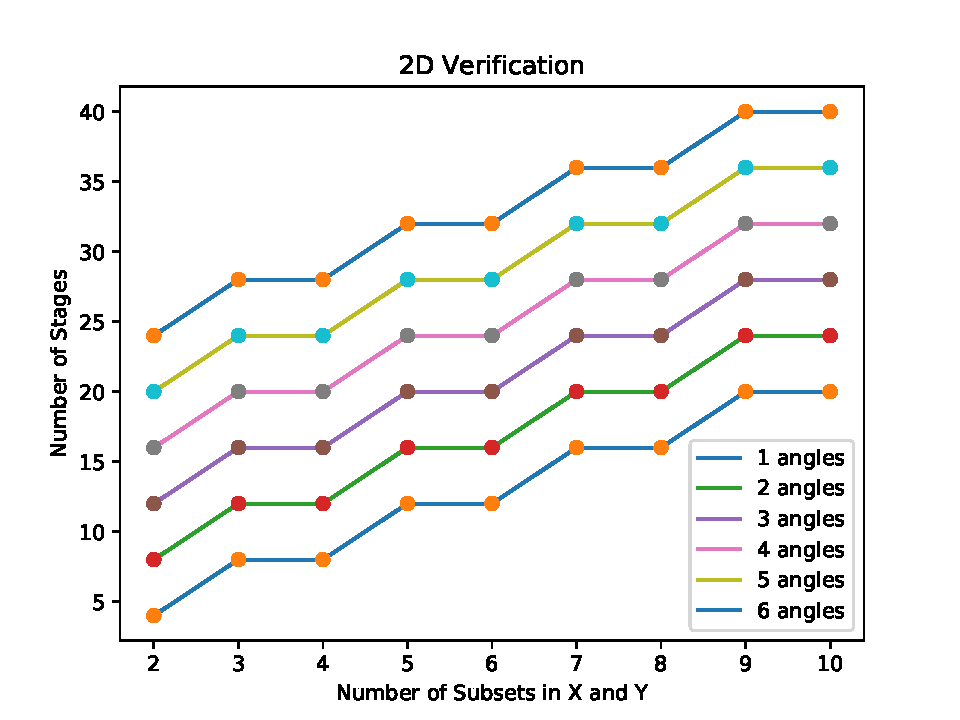
\includegraphics[scale=0.8]{../figures/regular_verification.pdf}
\caption{A 2D verification suite with regular partitions run from 2x2 to 10x10 subsets with each case being run from 1 to 6 angles per quadrant.}
\label{regular_verification}
\end{figure}

\subsection{Mildly Random Partitions}
%Mild random partitions
\begin{figure}[H]
\centering
\begin{subfigure}[b]{0.45\textwidth}
  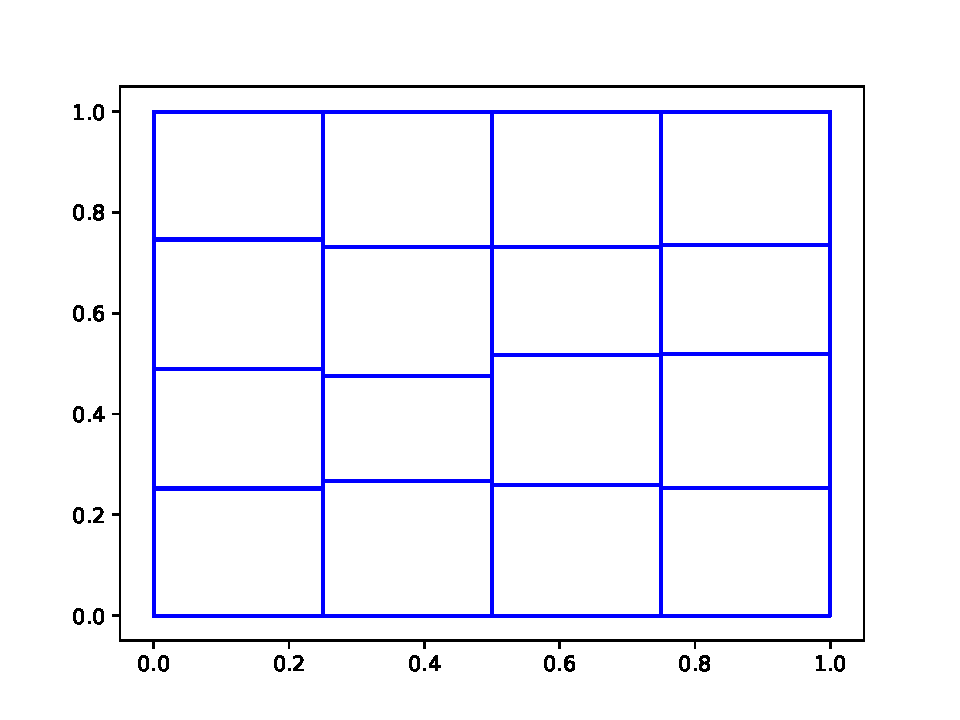
\includegraphics[width=\textwidth]{../cut_line_files/4_mild_random.pdf}
  \caption{4x4 subsets with mildly random partitions.}
  \label{4mildrandom}
\end{subfigure}
\begin{subfigure}[b]{0.45\textwidth}
  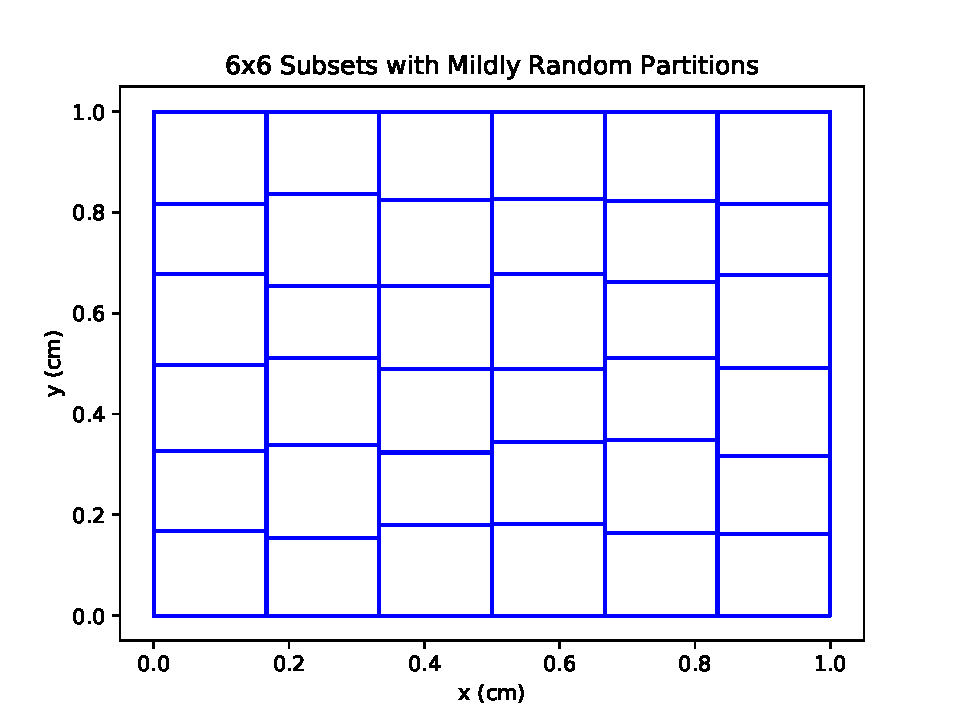
\includegraphics[width=\textwidth]{../cut_line_files/6_mild_random.pdf}
  \caption{6x6 subsets with mildly random partitions.}
  \label{6mildrandom}
\end{subfigure}

\begin{subfigure}[b]{0.45\textwidth}
  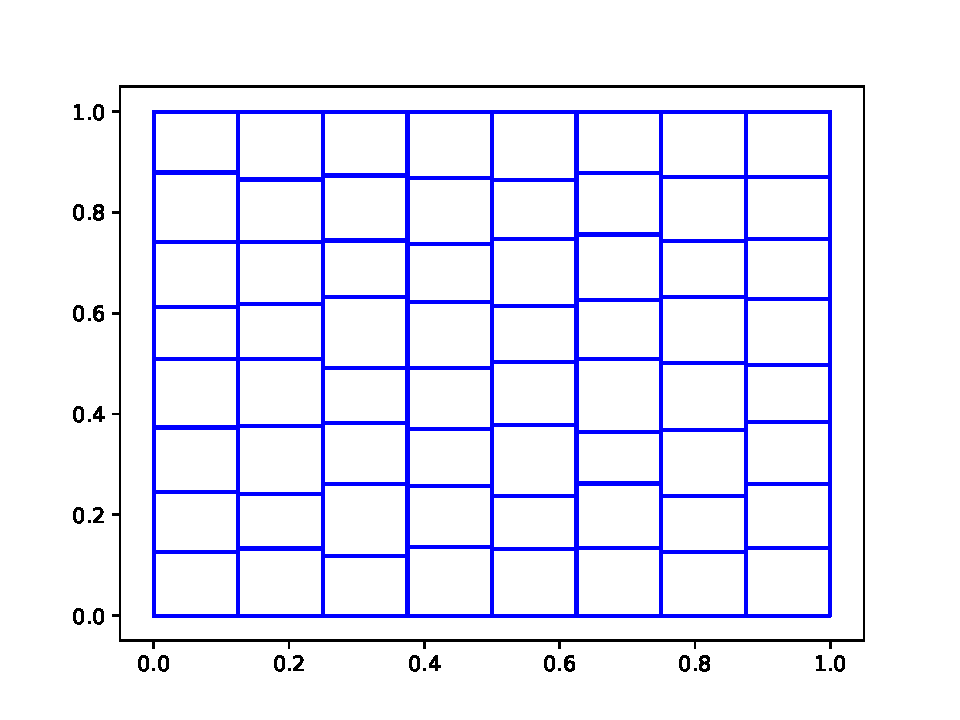
\includegraphics[width=\textwidth]{../cut_line_files/8_mild_random.pdf}
  \caption{8x8 subsets with mildly random partitions.}
  \label{8mildrandom}
\end{subfigure}
\begin{subfigure}[b]{0.45\textwidth}
  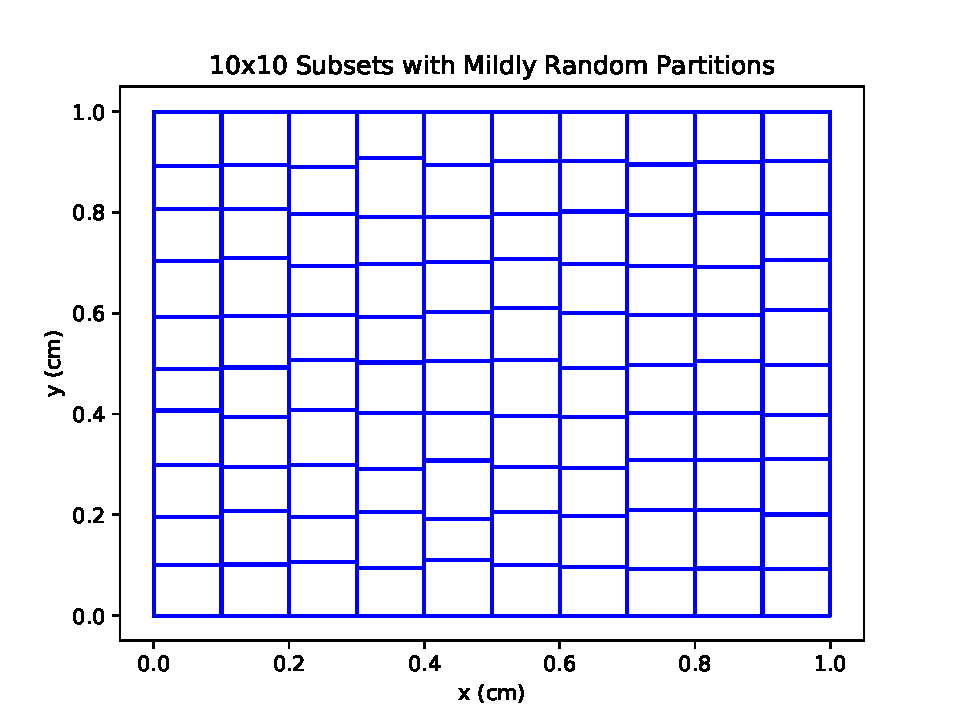
\includegraphics[width=\textwidth]{../cut_line_files/10_mild_random.pdf}
  \caption{10x10 subsets with mildly random partitions.}
  \label{10mildrandom}
\end{subfigure}
\caption{Examples of mildly random partitioning.}
\label{mild_random_partitions}
\end{figure}

\begin{figure}[H]
\centering
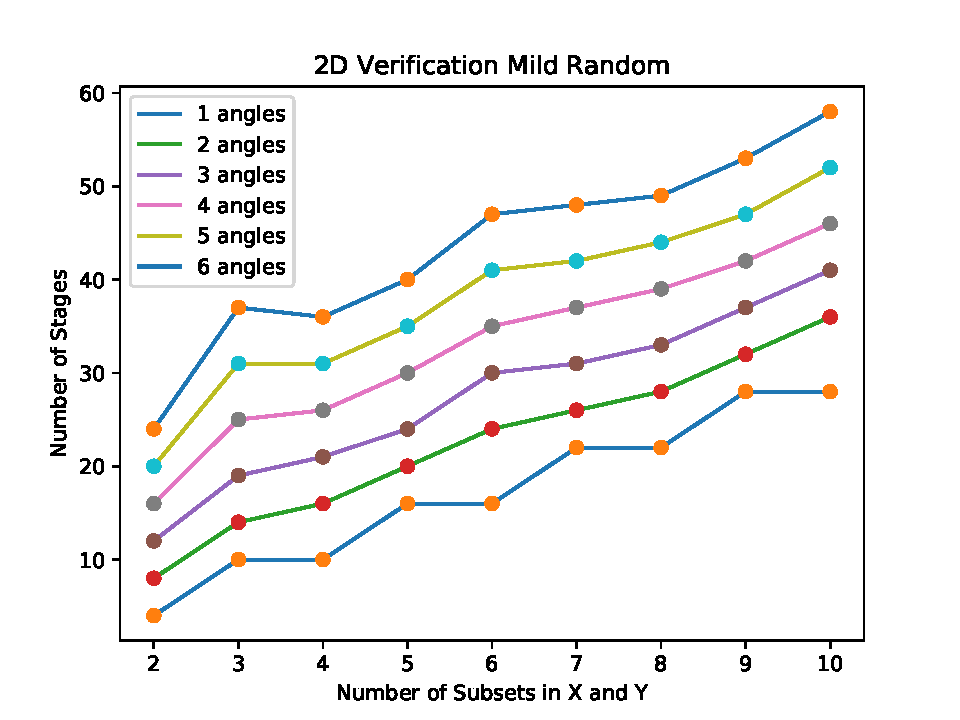
\includegraphics[scale=0.8]{../figures/mild_random_verification.pdf}
\caption{A 2D verification suite with mildly random partitions run from 2x2 to 10x10 subsets with each case being run from 1 to 6 angles per quadrant.}
\label{mild_random_verification}
\end{figure}

\subsection{Random Partitions}
%Random partitions
\begin{figure}[H]
\centering
\begin{subfigure}[b]{0.45\textwidth}
  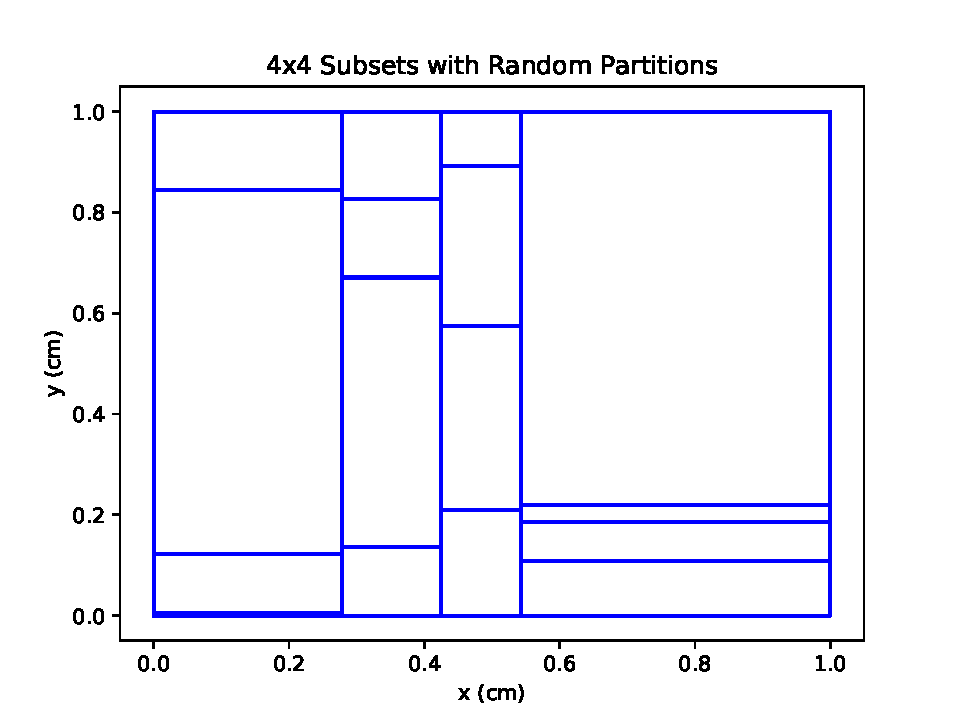
\includegraphics[width=\textwidth]{../cut_line_files/4_random.pdf}
  \caption{4x4 subsets with random partitions.}
  \label{4random}
\end{subfigure}
\begin{subfigure}[b]{0.45\textwidth}
  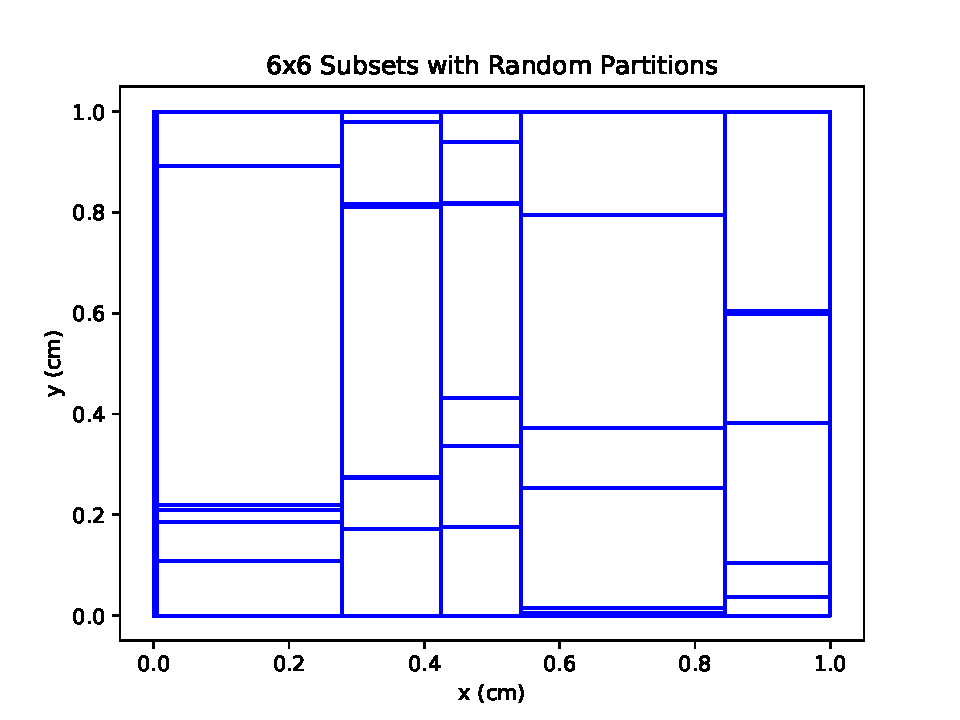
\includegraphics[width=\textwidth]{../cut_line_files/6_random.pdf}
  \caption{6x6 subsets with random partitions.}
  \label{6random}
\end{subfigure}

\begin{subfigure}[b]{0.45\textwidth}
  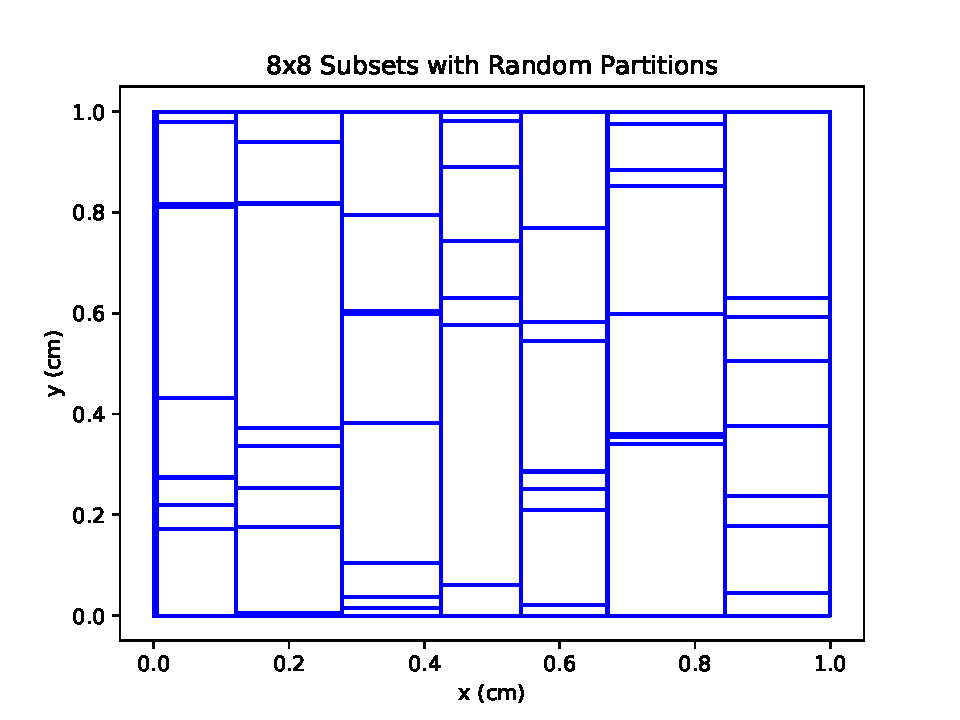
\includegraphics[width=\textwidth]{../cut_line_files/8_random.pdf}
  \caption{8x8 subsets with random partitions.}
  \label{8random}
\end{subfigure}
\begin{subfigure}[b]{0.45\textwidth}
  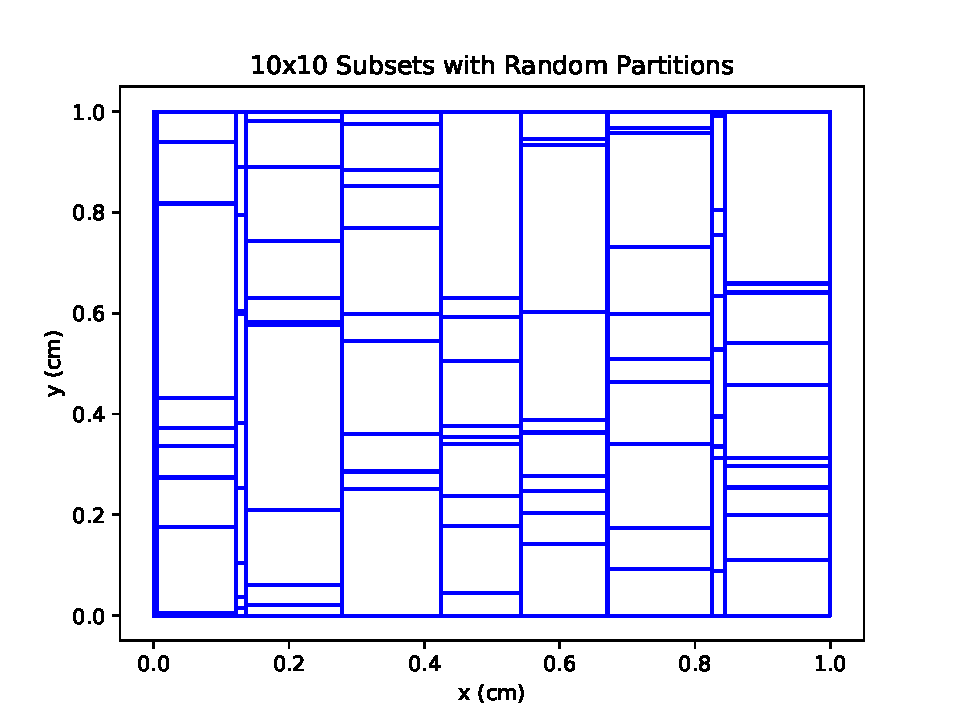
\includegraphics[width=\textwidth]{../cut_line_files/10_random.pdf}
  \caption{10x10 subsets with random partitions.}
  \label{10random}
\end{subfigure}
\caption{Examples of random partitioning.}
\label{random_partitions}
\end{figure}

\begin{figure}[H]
\centering
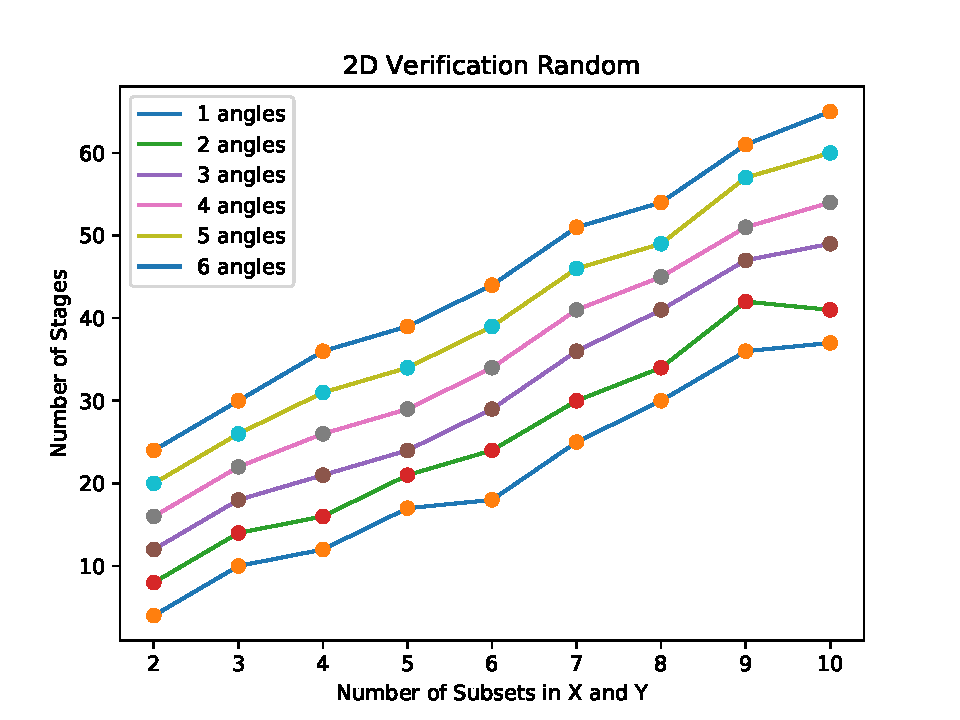
\includegraphics[scale=0.8]{../figures/random_verification.pdf}
\caption{A 2D verification suite with random partitions run from 2x2 to 10x10 subsets with each case being run from 1 to 6 angles per quadrant.}
\label{random_verification}
\end{figure}

\subsection{Probable Worst-Case Partitions}
\begin{figure}[H]
\centering
\begin{subfigure}[b]{0.45\textwidth}
  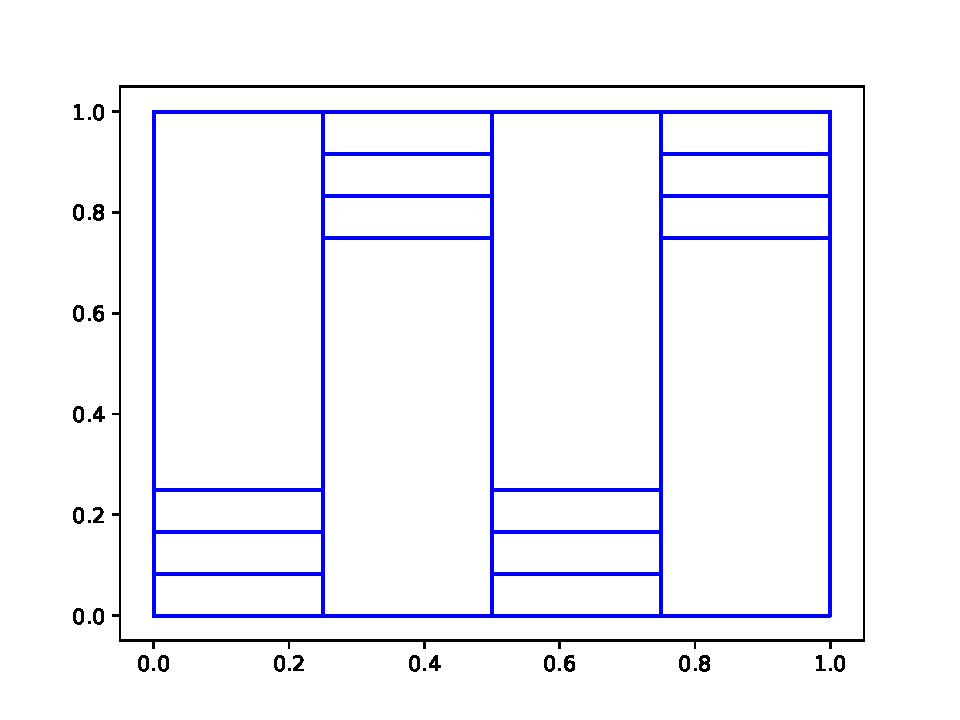
\includegraphics[width=\textwidth]{../cut_line_files/4_worst.pdf}
  \caption{4x4 subsets with probable worst-case partitions.}
  \label{4worst}
\end{subfigure}
\begin{subfigure}[b]{0.45\textwidth}
  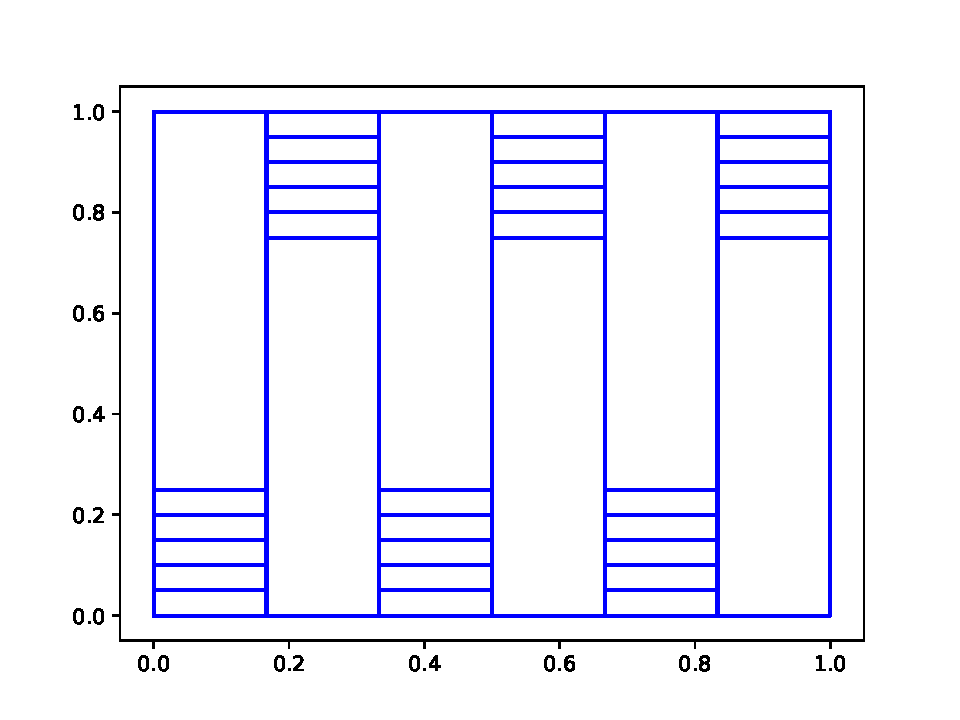
\includegraphics[width=\textwidth]{../cut_line_files/6_worst.pdf}
  \caption{6x6 subsets with probable worst-case partitions.}
  \label{6worst}
\end{subfigure}

\begin{subfigure}[b]{0.45\textwidth}
  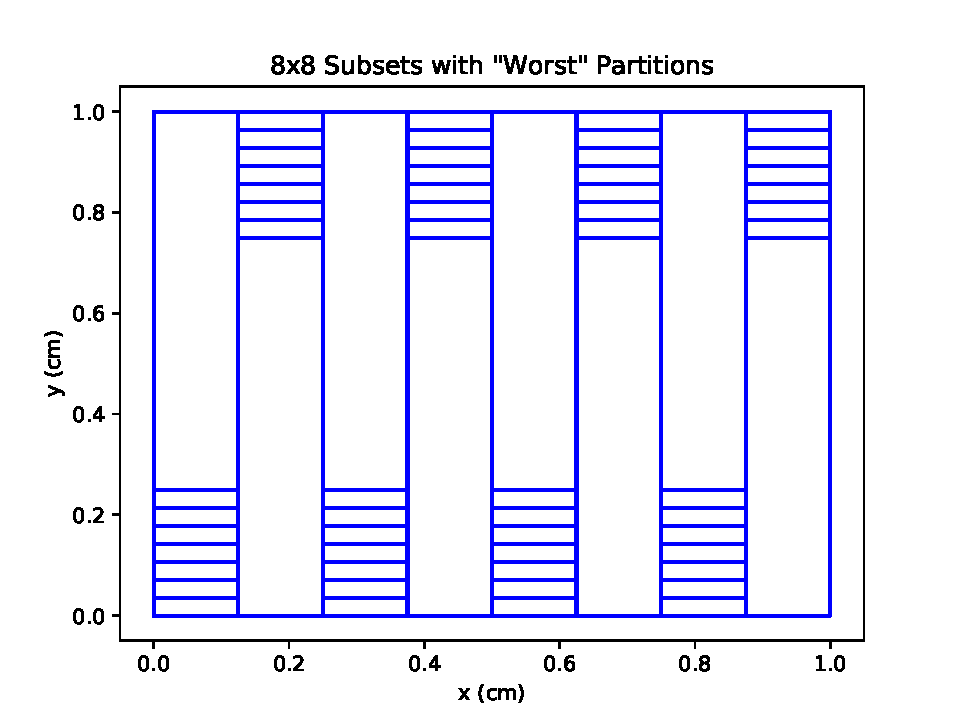
\includegraphics[width=\textwidth]{../cut_line_files/8_worst.pdf}
  \caption{8x8 subsets with probable worst-case partitions.}
  \label{8random}
\end{subfigure}
\begin{subfigure}[b]{0.45\textwidth}
  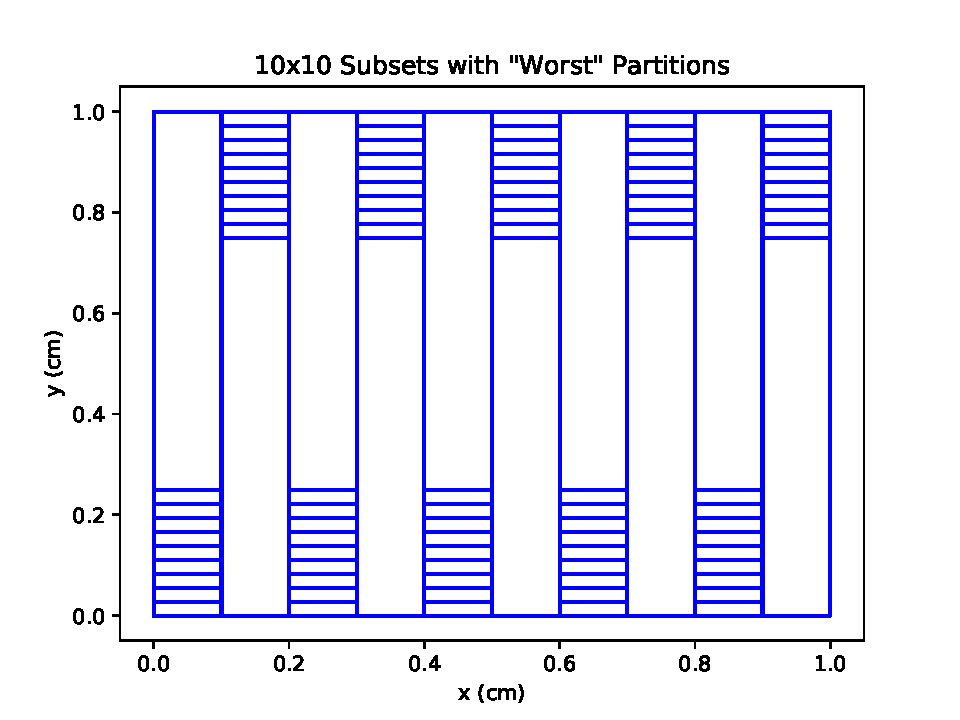
\includegraphics[width=\textwidth]{../cut_line_files/10_worst.pdf}
  \caption{10x10 subsets with probable worst-case partitions.}
  \label{10random}
\end{subfigure}
\caption{Examples of probable worst-case partitioning.}
\label{worst_partitions}
\end{figure}

\begin{figure}[H]
\centering
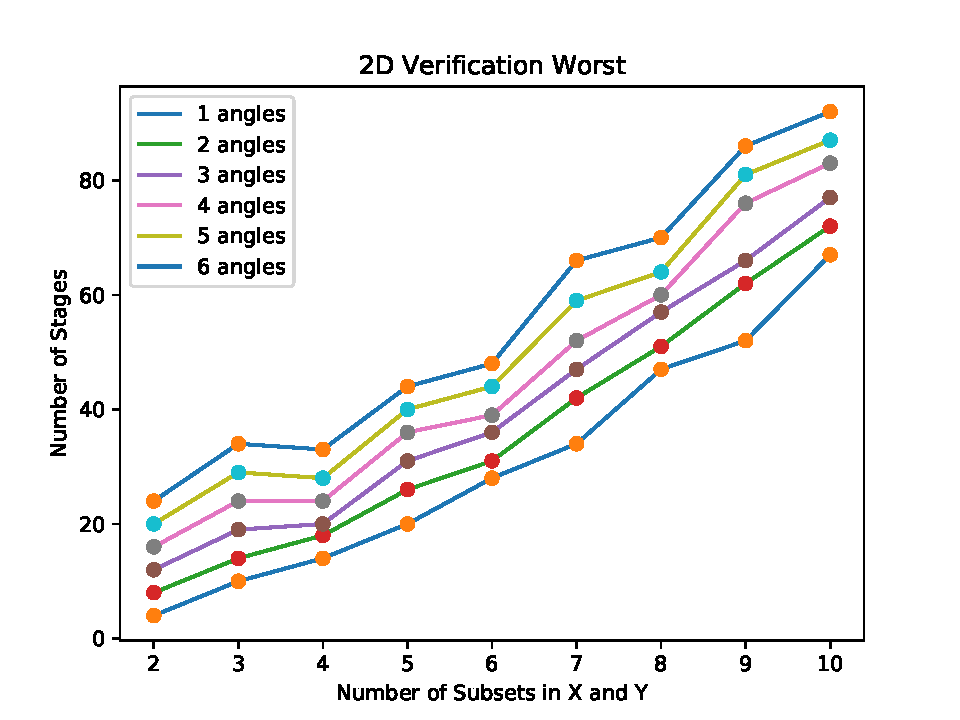
\includegraphics[scale=0.8]{../figures/worst_verification.pdf}
\caption{A 2D verification suite with probable worst-case partitions run from 2x2 to 10x10 subsets with each case being run from 1 to 6 angles per quadrant.}
\label{worst_verification}
\end{figure}

\section{3D Verification}

The 3d verification results will go here.
